\section{Результаты работы}

Программа реализована как консольная утилита, в параметрах запуска можно задать значение параметра натяжения для всех интервалов (если они не указаны во входных данных), число итераций по изменению натяжения, значение параметра релаксации (по умолчанию --- 1), формат вывода --- формулы сегментов (по умолчанию) или скрипт для \texttt{gnuplot}.

Демонстрация текстового вывода:
\footnotesize\begin{alltt}
$ ./main -p 10 -tense 1 -relax 0.5 < tests/sin.txt
[0.3927:1.1781] (0 * sinh(10 * (1.1781 - x)) + 15.8202 * sinh(10 * (x - 0.3927))) / 128801 + 0.5 * (1.1781 - x) / 0.7854 + -0.658202 * (x - 0.3927) / 0.7854
[1.1781:1.9635] (15.8202 * sinh(10 * (1.9635 - x)) + -16.9673 * sinh(10 * (x - 1.1781))) / 128801 + -0.658202 * (1.9635 - x) / 0.7854 + 0.669673 * (x - 1.1781) / 0.7854
[1.9635:2.7489] (-16.9673 * sinh(10 * (2.7489 - x)) + 16.9673 * sinh(10 * (x - 1.9635))) / 128801 + 0.669673 * (2.7489 - x) / 0.7854 + -0.669673 * (x - 1.9635) / 0.7854
[2.7489:3.5343] (16.9673 * sinh(10 * (3.5343 - x)) + -15.8202 * sinh(10 * (x - 2.7489))) / 128801 + -0.669673 * (3.5343 - x) / 0.7854 + 0.658202 * (x - 2.7489) / 0.7854
[3.5343:4.3197] (-15.8202 * sinh(10 * (4.3197 - x)) + 0 * sinh(10 * (x - 3.5343))) / 128801 + 0.658202 * (4.3197 - x) / 0.7854 + -0.5 * (x - 3.5343) / 0.7854
\end{alltt}
\normalsize

\begin{figure}[h]
\centering
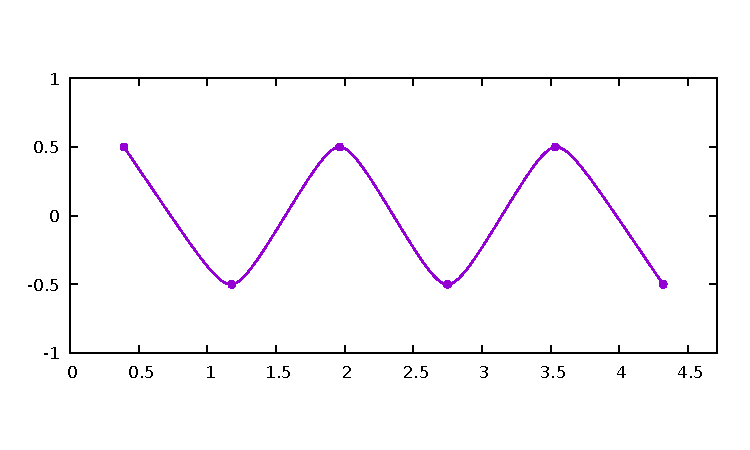
\includegraphics{sin}
\caption{Предыдущий тестовый пример}
\end{figure}

\begin{figure}[t]
\centering
\subfigure[]{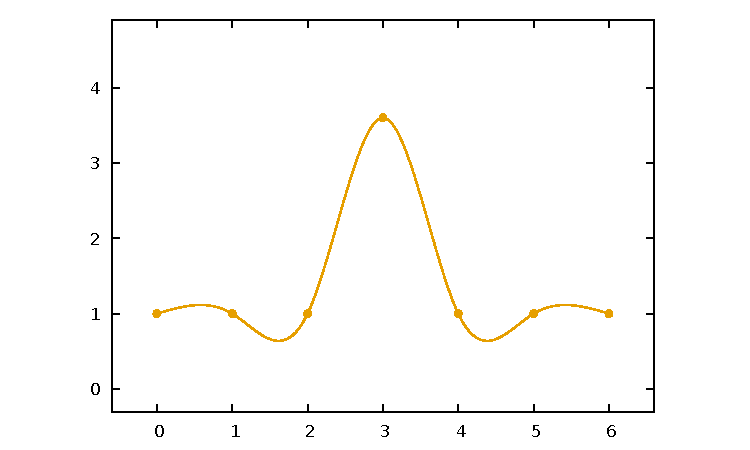
\includegraphics[width=.5\textwidth]{outlier_cub}}\hfill
\subfigure[]{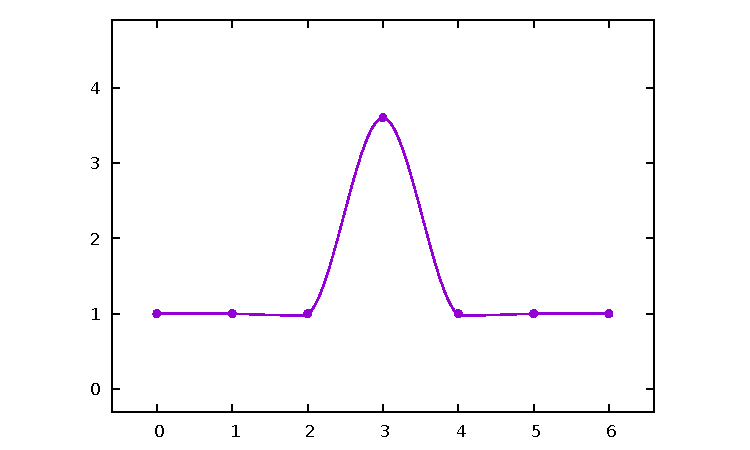
\includegraphics[width=.5\textwidth]{outlier_exp}}
\caption{Пример с выпавшей точкой. (a) Кубический сплайн. (b) Экспоненциальный сплайн (параметры натяжения подобраны вручную)}
\end{figure}

\begin{figure}[t]
\centering
\subfigure[]{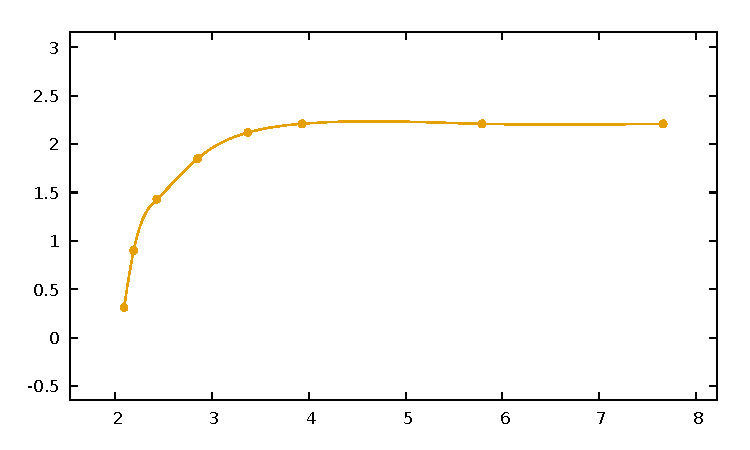
\includegraphics[width=.5\textwidth]{vert_tangent_cub}}\hfill
\subfigure[]{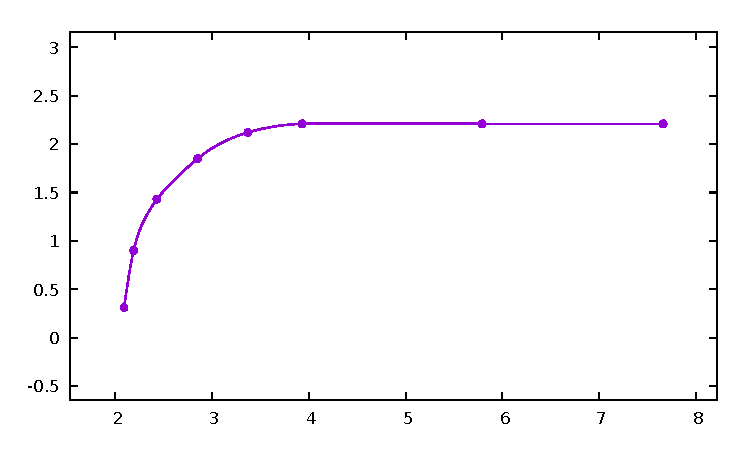
\includegraphics[width=.5\textwidth]{vert_tangent_exp}}
\caption{Пример с вертикальным наклоном. (a) Кубический сплайн. (b) Экспоненциальный сплайн (параметры натяжения подобраны частично вручную, частично итеративным методом)}
\end{figure}
\FloatBarrier

\begin{figure}[h]
\centering
\subfigure[]{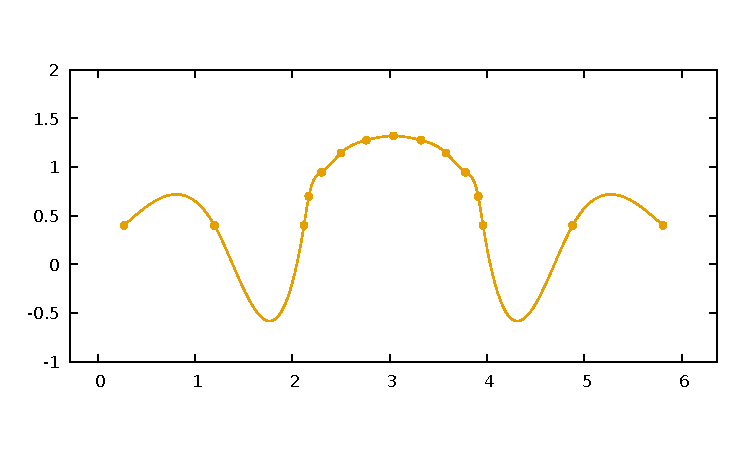
\includegraphics[width=.5\textwidth]{semicircle_cub}}\hfill
\subfigure[]{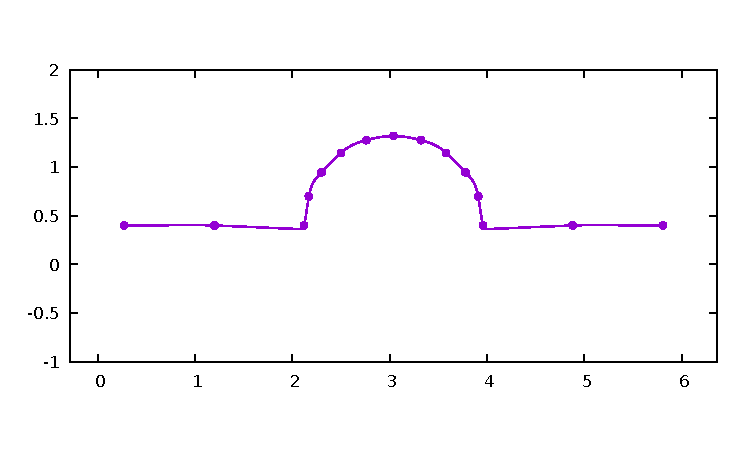
\includegraphics[width=.5\textwidth]{semicircle_exp}}
\caption{Пример с разрывом наклона. (a) Кубический сплайн. (b) Экспоненциальный сплайн (параметры натяжения подобраны частично вручную, частично итеративным методом)}
\end{figure}

\begin{figure}[h]
\centering
\subfigure[]{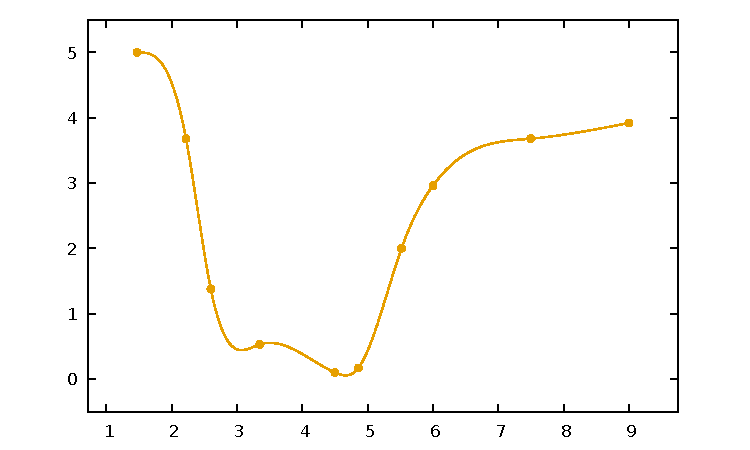
\includegraphics[width=.5\textwidth]{curve_cub}}\hfill
\subfigure[]{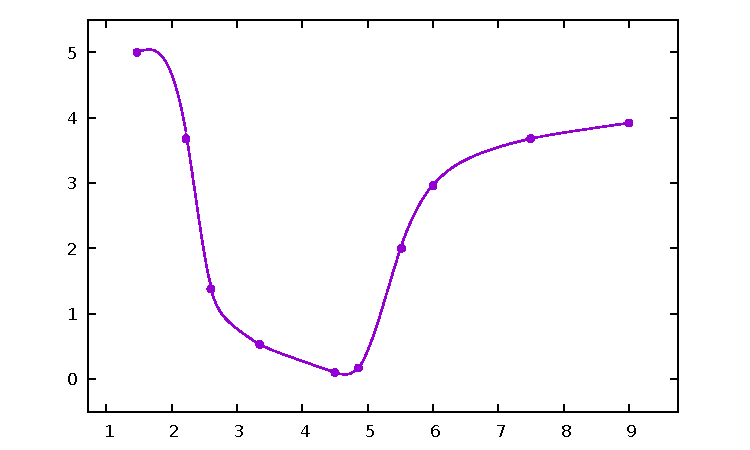
\includegraphics[width=.5\textwidth]{curve_exp}}
\caption{Пример с ложными точками перегиба. (a) Кубический сплайн. (b) Экспоненциальный сплайн (параметры натяжения подобраны итеративным методом)}
\end{figure}

\begin{figure}[h]
\centering
\subfigure[]{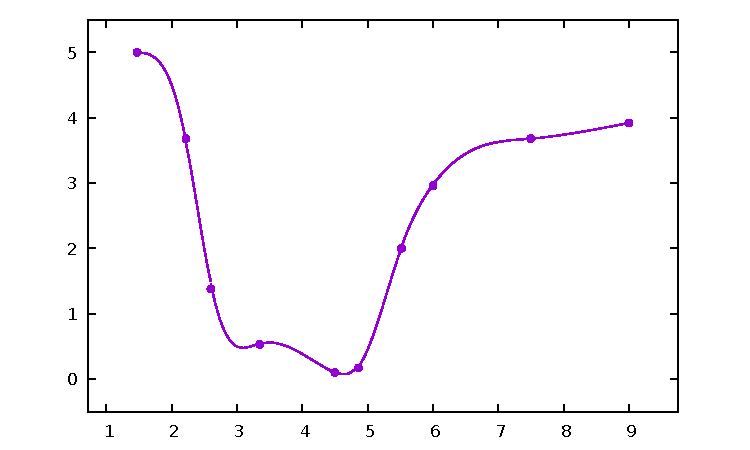
\includegraphics[height=.28\textheight]{curve_exp_0}}
\subfigure[]{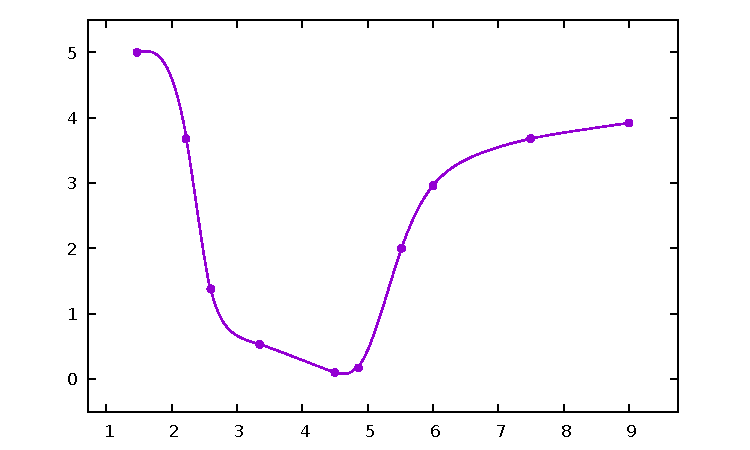
\includegraphics[height=.28\textheight]{curve_exp_1}}
\subfigure[]{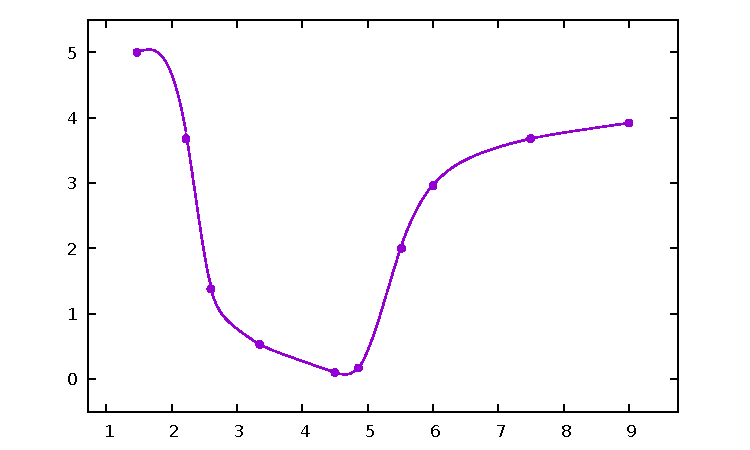
\includegraphics[height=.28\textheight]{curve_exp_2}}
\caption{Пример с ложными точками перегиба. (a) Нулевая итерация. (b) Первая итерация. (c) Вторая итерация}
\end{figure}
\FloatBarrier

\pagebreak
